\section{Background and Motivation}
\label{s:background}

% In this section, we briefly describe the basics of volumetric video before   describing the motivation for \livo. 

\parab{Volumetric Video.}
%
Volumetric video captures a three-dimensional representation of a continuously evolving scene (\eg a game, a live performance, a conference call).
%
Each viewer of a volumetric video has 6 degrees of freedom (6DoF)~---~he/she can view the video from any point in the captured space, in any direction.
%
For example, a viewer can watch a live performance of a string quartet as though sitting next to a violinist, while at the same time, another viewer can take the cellist's perspective.
%
Or, a technician can remotely assist debugging and repairing an aircraft part, moving in space to inspect the part from different perspectives.
%\agr{Remote assist for debugging an ASML machine without flying a technician might be easier to buy.  Collaborative music would be awesome, but tough with the current lag}
%
Typically, viewers watch volumetric videos on a mixed-reality headset.
%
They \emph{interact} with the video by moving around in a physical space; the headset tracks the viewer's movement and, at any given moment, renders the video from a perspective consistent with the viewer's current position and orientation.
%
%% \begin{figure}[t]
%%   \begin{minipage}[t]{0.32\columnwidth}
%%     \centering
%%      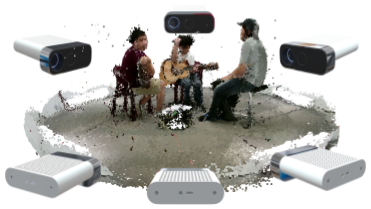
\includegraphics[width=\columnwidth]{figures/capture.png}
%%     \caption{Capture}
%%     \label{plot:capture}
%%   \end{minipage}
%%   \begin{minipage}[t]{0.32\columnwidth}
%%     \centering
%%      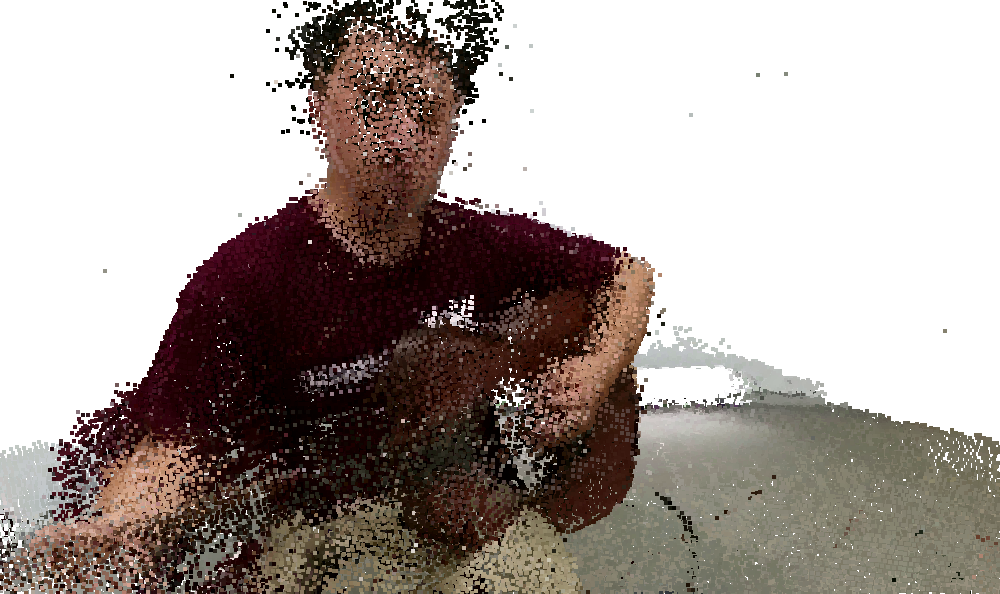
\includegraphics[width=\columnwidth]{figures/1400.png}
%%     \caption{Viewpoint 1}
%%     \label{plot:rendered-view1}
%%   \end{minipage}
%%   \begin{minipage}[t]{0.32\columnwidth}
%%     \centering
%%      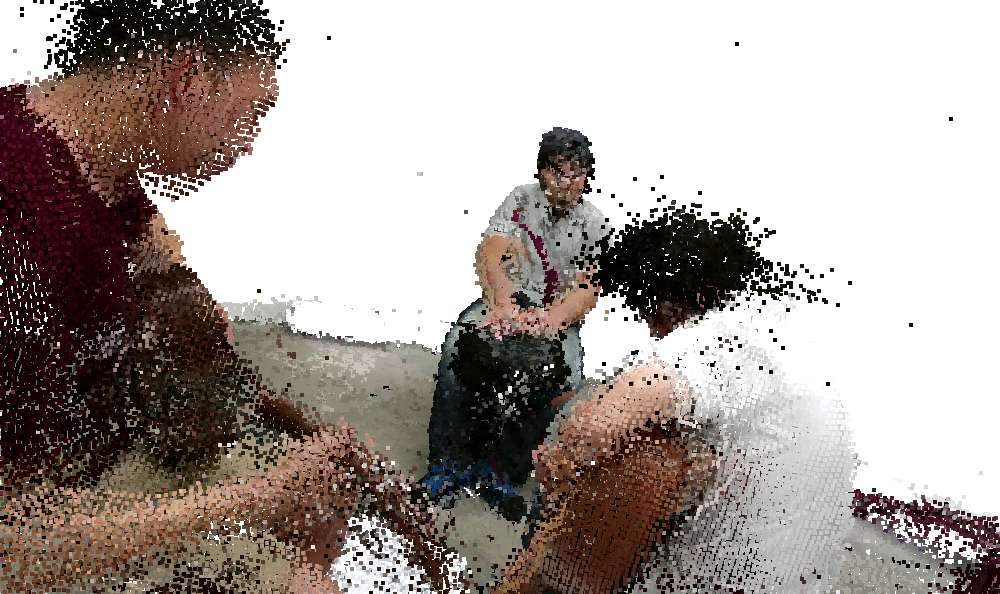
\includegraphics[width=\columnwidth]{figures/1470.png}
%%     \caption{Viewpoint 2}
%%     \label{plot:rendred-view2}
%%   \end{minipage}
%% \end{figure}
%
\begin{figure}[t]
     \centering
     \begin{subfigure}[t]{0.32\textwidth}
         \centering
         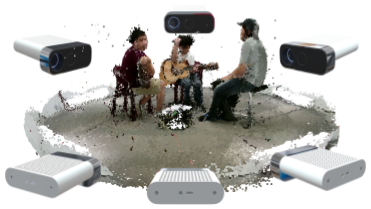
\includegraphics[width=\textwidth]{figures/capture.png}
         % \caption{$y=x$}
         \label{fig:y equals x}
     \end{subfigure}
     \hfill
     \begin{subfigure}[t]{0.32\textwidth}
         \centering
         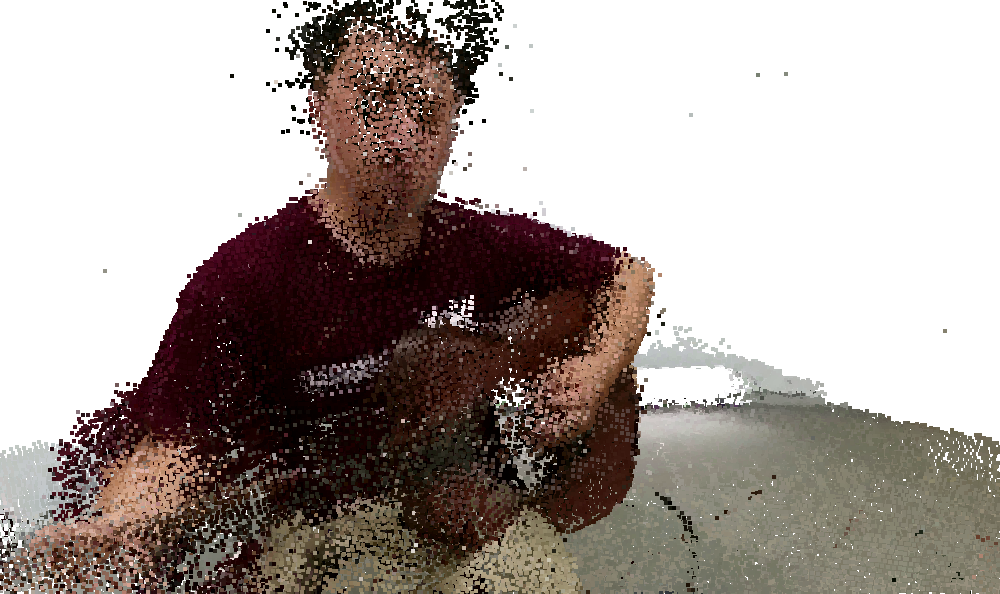
\includegraphics[width=\textwidth]{figures/1400.png}
         % \caption{$y=3\sin x$}
         \label{fig:three sin x}
     \end{subfigure}
     \hfill
     \begin{subfigure}[t]{0.32\textwidth}
         \centering
         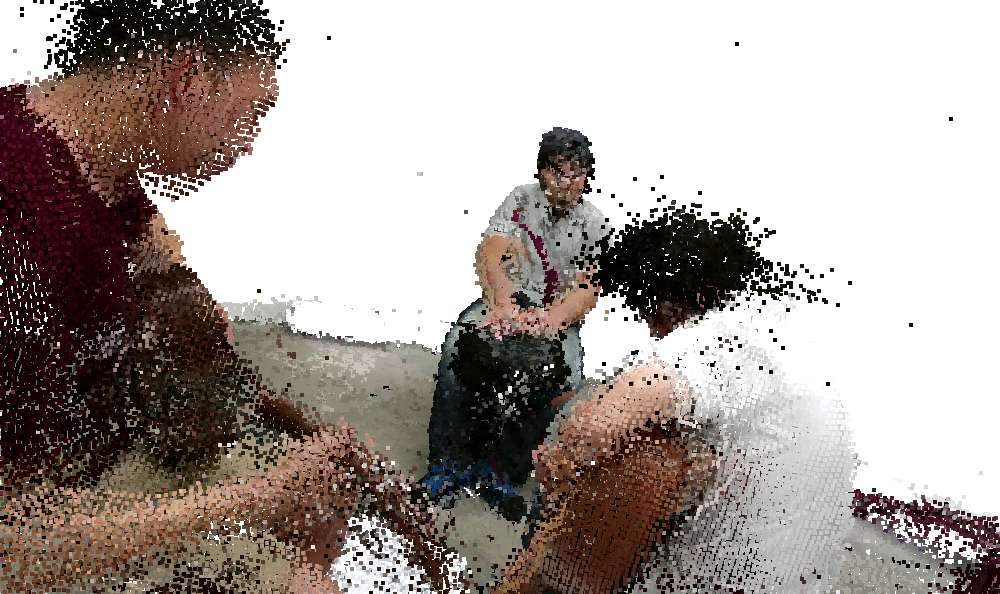
\includegraphics[width=\textwidth]{figures/1470.png}
         % \caption{$y=5/x$}
         \label{fig:five over x}
     \end{subfigure}
        \caption{\textbf{Left:} Capture, \textbf{Right:} Two user viewpoints from an actual user trace.}
        \label{fig:3D_example}
\end{figure}
%
Thus, in our example of the musical performance, viewers can move to change perspective during the performance (\cref{fig:3D_example}).
%\ramesh{Consider adding a figure to show an RGB-D array surrounding a performance, and maybe show two different perspectives at the same time}

A volumetric video consists of a sequence of 3D frames, each representing a three-dimensional capture of a physical space.
%
A \emph{point cloud}~\cite{vivo, groot} is one representation of a frame; we discuss another, the \textit{mesh}, later.
%
Each point in a point cloud corresponds to a 3D location (usually on the surface of an object) that has location coordinates (also called \textit{geometry}) and color of the surface at that location.
%
%Collectively, then, points in a point cloud capture the \emph{geometry} and \emph{color} of a scene in three dimensions. %\raj{Do we need to differentiate briefly with lidar point clouds with no color? Perhaps the angle that one is for downstream computation while color ptcl is for vieweing.}
% \rn{Other reasons to focus on point clouds? I added popularity but perhaps generation overheads also matter?}

In this paper, we consider volumetric videos obtained from an array of off-the-shelf RGB-D cameras encircling a scene.
%\ramesh{If space permits, add a graphic for this as part of the earlier figure.}
% 
Commodity RGB-D cameras, such as Azure Kinect DK~\cite{kinect} or Intel RealSense~\cite{realsense}, can capture both the color (RGB) and depth (D) of points in a scene.
%
% For example, the Kinect estimates depth using Time-of-flight~---~the time taken to receive the reflection of an emitted infrared beam.
%
By aligning (\cref{ss:compression}) RGB-D frames from multiple cameras, one can estimate the position and color of an arbitrary point in the scene, thereby generating a point cloud.
%
% Over the past few years, RGB-D cameras have become cheap enough that they are now a popular way to capture volumetric videos~\cite{depthkit}.

% A volumetric video is a seqeunce of 3D captures represented explicitly as point clouds (ptcl)~\cite{cite:vivo, cite:groot} or meshes~\cite{cite:meshreduce}, implcitly represented using NeRFs~\cite{cite:nerf}. Out of these, point cloud have become quite popular, due to it's simplicity and flexibility. For every frame in a volumetric video, a point cloud is generated from RGB-D captures from multiple cameras (typically >$3$) synchronized together. Kinect synchronizes color and depth internally, while it uses external signal via 3.5-mm synchronization port, which the master camera uses to instruct the subordinate cameras to capture together. 

% \parab{Ptcl Generation.}
% Each synchronized color and depth frame from a camera is projected in 3D to form a point cloud using the camera's \textit{instrinsic parameters}. The point cloud is generated in the camera's local coordinate system by the following:
% \raj{Give the math behind point cloud generation.}
% A complete frame of volumetric video is generated by stitching the local point clouds from each camera in global coordinate system. Each of the camera's global position and rotation is estimated using extrinsic camera calibration methods~\cite{cite:zhang}~\cite{cite:icp}. Each point from the local point cloud is projected to the global coordinates by translation and rotation as obtained by the local camera's \textit{extrinsic parameters}. This is performed for all the points across all the cameras to form the stiched point cloud. A sequence of such sticted point clouds form a volumetric video.

%% \antonio{Nice table.}

\parab{Truly Immersive Two-Way Conferencing.}
%
We consider the problem of streaming volumetric video between two locations (\textbf{A} and \textbf{B}) while permitting 6-DoF viewing at both ends.
%
In contrast to prior work~\cite{starline,farfetchfusion,tele-aloha} on volumetric video conferencing that transmits 3D representations of a single human being (their face or torso), we seek to stream a \textit{full-scene} from \textbf{A} that may consist of multiple participants and objects surrounding them (\eg furniture, the floor, walls, etc.).
%
Full-scene conferencing would enable an application in which, for example, groups of actors at \textbf{A} and \textbf{B} could collaborate jointly to rehearse an upcoming theater performance.
%
As users at \textbf{B} receive and view the video, they can move around the scene to change their perspective, permitting true immersion.
%
%\raj{6DoF allows users to have natural conversation as if they are same real-life scene. Should we differentiate early on that current systems like Starline and FarfetchFusion enjoy 3D conferencing but users are remain seated by design, thereby restricting 6DoF?}
%
These movements are captured in video transmitted to \textbf{A}, bringing a level of interactivity for human interaction comparable to physical presence.
%
%% \raj{Why do we need to transmit 6DoF information from B to A? It is only required for culling, but here we are making the point about interactivity in volumetric video.}\ramesh{No, the sentence is not talking about 6DoF information. It tries to say that, as the user at B moves, their cameras capture the movement and transmit it to A. Please review and/or fix.}\antonio{The main point here is two-way vs one-way, two sets of cameras each capturing users with HMDs. In addition to clarifying this in the text it would be good to think of an application that would require this. While the concert example makes sense it is one-way, and I'm not sure what would be a compelling two-way example.  }

To realize this interactivity, a conferencing system must
(a) transmit full-scene point clouds at \textit{full frame rate} (30 frames per second) (b) with an end-to-end latency of 200-300~ms~\cite{videoconf-benchmark,salsify,converge-sigcomm-2023,rfec-acm-mm2022}. 
%
Today's 2D conferencing systems satisfy these requirements.
%
Full-scene point clouds can be much larger than those representing more constrained views (single human beings with only their face or torso).
%
For example, in one 3D dataset~\cite{panoptic} we use in \cref{s:evaluation}, the average point cloud frame size for a participant (single human in the scene) is about 1~MB uncompressed, but for the full-scene (with furnitures, floor, objects, \etc) is 10~{MB} (\cref{tab:dataset-summary}).
%
As such, transmitting full-scenes will require significant network bandwidth.
%
Today, average global broadband speeds are nearly 100~Mbps and are expected to increase by 20\% annually~\cite{cisco_whitepaper}; thus, we expect immersive two-way conferencing to be feasible in the near future, if it is not already.

% \begin{table}[t]
%   \begin{tabular}{|l|l|} \hline
%     \textbf{Prior Work} & \textbf{Avg. Point Cloud Size (MB)} \\ \hline
%   \end{tabular}
%   \caption{Point cloud sizes used in prior work, compared to ours}
%   \label{tab:sizes}
% \end{table}

\begin{table}[t]
 \begin{center}
{%\footnotesize
  % \scalebox{0.7}
  {
  \begin{tabular}{|l|l|l|l|l|l|l|}
    \hline
    \textbf{\begin{tabular}[c]{@{}l@{}}Streaming \\ Systems\end{tabular}} & \textbf{Type} & \textbf{\begin{tabular}[c]{@{}l@{}}Compress-\\ ion\end{tabular}} & \textbf{Content} & \textbf{\begin{tabular}[c]{@{}l@{}}BW-\\ adaptive?\end{tabular}} & \textbf{FPS} & \textbf{Cull?} \\ \hline
    ViVo~\cite{vivo} & On-demand & 3D & Multiple Person & Indirect & 30 & \checkmarkk \\ \hline
    Groot~\cite{groot} & On-demand & 3D & Full-scene & No & 30 & \checkmarkk \\ \hline
    Fumos~\cite{fumos} & On-demand & 3D & Single Person & No & 30 & \checkmarkk \\ \hline
    Vues~\cite{vues} & On-demand & 2D & Multiple Person & Indirect & 30 & \checkmarkk \\ \hline
    Holoportation~\cite{holoportation} & Conferencing & 3D & Single Person & No & 30 & \crossmark \\ \hline
    LiveScan3D~\cite{livescan3d} & Live & 3D & Full-scene & No & 15 & \crossmark \\ \hline
    FarFetchFusion~\cite{farfetchfusion} & Live & 2D & Portrait & No & 30 & \crossmark \\ \hline
    Starline~\cite{starline} & Conferencing & 2D & Upper Torso & No & 30 & \crossmark \\ \hline
    Tele-Aloha~\cite{tele-aloha} & Conferencing & 2D & Upper Torso & No & 30 & \crossmark \\ \hline
    VRComm~\cite{vrcomm} & Conferencing & 2D & One Person & No & 30 & \crossmark \\ \hline
    MeshReduce~\cite{meshreduce} & Live & 3D & Full-scene & Indirect & 15 & \crossmark \\ \hline
    MetaStream~\cite{metastream} & Live & 3D & One Person & No & 30 & \crossmark \\ \hline
    \rowcolor{Gainsboro!60} \livo & Conferencing & 2D & Full-scene & Direct & 30 & \checkmarkk \\ \hline
    \end{tabular}
  }
}
  \caption{Comparison to related work, more details in \cref{ch:related}.}
  \label{tab:comparison}
  %\vspace{-3mm}
\end{center}
\end{table}

\parab{Challenge: Compression.}
%
Even with increased broadband speeds, transmitting full-scenes will require compression.
%
In our example above, each full frame needs to be compressed to over a twentieth of its original size to fit the 100~Mbps capacity.
%
%% \raj{10~MB frame at 30 fps, produces $10\times8\times30=2400$~Mbps. So, we need to compress $1/24$ times of its original size to fit.}
%
The need for compression is unlikely to go away: even if broadband bandwidth increases, point cloud sizes might increase with better cameras.

Point cloud compression techniques such as Draco~\cite{draco}, V-PCC~\cite{vpcc}, and G-PCC~\cite{gpcc} can potentially address this.
%
Indeed, prior work has used one or more of these for on-demand~\cite{groot,vivo} and live~\cite{metastream} streaming of non-full-scene volumetric video.

However, these techniques can be compute intensive and their computational complexity grows linearly with point cloud size. %because they construct spatial indices (k-d trees or octrees) for each point cloud for intra-frame (within point cloud) or inter-frame (between successive point clouds) compression.
%
%The computational complexity of these compression techniques scales linearly with point cloud size.
%
For example, on a machine we use in \cref{s:evaluation}, compressing a 1~MB point cloud using Draco takes 25~ms while compressing a 10~MB frame takes over 300~ms.
%
Other compression techniques are slower: 8 minutes using V-PCC for 11~MB point clouds, and 10 seconds for G-PCC.
%
%% \raj{We have our own numbers for V-PCC and G-PCC on few frames in `band2`. Use those numbers here? Do we need a table like Table 2 in ViVo and Groot?}\ramesh{No need for a table, but yes please replace this with our numbers.}
%
These latencies can make it difficult, if not impossible, to achieve the 200-300~ms end-to-end latency target discussed above.
%
Parallelizing compression~\cite{vivo,metastream,meshreduce} can help, but the increase in compute cost can deter or delay adoption. %\rn{is there a reason we have to keep compute so low given that these are servers?}
%
%% \raj{Ravi made a point earlier~---~``Is there a reason we have to keep compute so low given that these are servers?''. Reason why server needs to have low compute is because 2-way conferencing makes the server also a receiver.}\ramesh{So that's why we talk about compute cost, which can be significant. Do we need to elaborate more?}
%Beyond compression latencies

Point cloud compression techniques also do not achieve as high compression efficiencies as 2D video compression.
%
This is because their \textit{inter-frame} compression algorithms are the subject of ongoing research~\cite{pcc-future,hong2022motion,hong2022fractional}.
%
For instance, Draco's default setting can compress the 10~MB per full-frame video to about 1.78~MB per frame.
%
In contrast, the approach we describe in this paper does not use point cloud compression and can compress to about 0.66~MB per frame on average.
%% \antonio{We need to be aware of and address the following limitation; VPCC can take any point cloud and map to 2D video, no matter how it was captured or generated (it does have the complexity limitation that is mentioned in the text, but it also has some of the advantages of working with 2D video). Instead, the proposed method assumes that the 2D video used to create the point cloud is available. This is a reasonable assumption, but it also means that our method cannot be used on existing point clouds; it applies only to systems where one has access to the individual 2D video cameras.}
%% \antonio{For a comparison of this type one would want to have rate-distortion plots. Also, depending on the metric (e.g., PSNR vs SSIM) describing the drop in performance in terms of percentage may not be appropriate. }

\parab{Challenge: Bandwidth-adaptivity.}
%
Even with increasing average bandwidths, it will be important for two-way conferencing to be \textit{bandwidth-adaptive}.
%
Bandwidth availability can vary spatially (\ie across different regions) and temporally (\ie during a single session).
%
Two-way conferencing can exploit high bandwidth availability to deliver high quality.
%
However, when bandwidth drops, it must deliver volumetric video without stalling.
%
%% \antonio{Previous sentence is not very clear.
%% %
%% Maybe just shorten the sentence and make the point that it's important to avoid stalling in two-way live streaming?}

2D video conferencing systems (e.g., those that use WebRTC~\cite{webrtc}) address this by (a) continuously estimating available bandwidth and (b) using a \textit{rate-adaptive} codec implementation.
%
Such a codec takes a desired bandwidth as input, and attempts to encode the frame at that target bandwidth, thus \textit{directly} adapting to bandwidth changes.
%
Today, compression algorithm implementations that directly compress point clouds or meshes (\eg Draco~\cite{draco}) are \textbf{not} rate-adaptive: applications cannot specify a target output bitrate when compressing 3D frames.
%
Instead, they contain parameters that control the \textit{quality} of the encoder output.
%
For example, Draco's \textit{quality parameter} (QP) governs the degree of allowable distortion in the output; lower quality output requires lower rate for transmission.
%
However, given a target available bandwidth, an application cannot know \textit{a priori} what QP value to choose to achieve that bandwidth.
%
Recent work, MeshReduce~\cite{meshreduce}, profiles 3D videos offline to develop a mapping from bitrate to one or more parameters (like QP).
%
During a session, given the current available bandwidth, it instructs the compression algorithm to use parameters from the mapping.
%
This approach can only \textit{indirectly} adapt to bandwidth (as opposed to using a codec implementation that can directly encode at a given target rate).
%
It can also be conservative: as \cref{tab:mahimahi-traces} shows, unlike \livo{} which uses direct bandwidth adaptation, MeshReduce produces encodings that are significantly lower than the target bandwidth.
%
As a result, it has lower perceptual and objective quality (\cref{s:evaluation}).

%% Unlike a rate-adaptive codec that permits \textit{direct} bandwidth-adaptivity, indirect adaptation can result in output rates that are significantly different from the current available bandwidth.%\agr{I'm confused about direct vs indirect...}
%% %
%% This occurs because the profiles don't generalize well to all videos and because profiles capture average behavior but individual frames can deviate significantly from the average.
%% %
%% To quantify this, \cref{fig:dir-indir} shows the results of an experiment in which we apply indirect bandwidth adaptation to a 3D video.
%% %
%% Specifically, for the purpose of illustration, we attempt to encode the entire video to a single, fixed, bitrate.
%% %
%% Unfortunately, indirect adaptation results in widely varying output bitrates, which can induce stalls and adversely impact quality.
%% %
%% In contrast, the approach we develop in this paper, \livo{}, uses \textit{direct} bitrate adaptation, which produces rates that more closely target the desired available bandwidth (\cref{fig:dir-indir}), while automatically adapting to scene complexity changes.
%% %
%% %% \raj{Add to the last line in the para that it generalizes to new scenes and changes to scene complexity within the scene. Also, I felt that we haven't explained the term ``scene complexity'' very well.}
%% \antonio{I find the discussion of direct and indirect adaptation above very confusing; perhaps better terms could be useful. If I understood correctly by ``direct'' you mean ``real-time'' since the bit rate changes during transmission, but ``indirect'' involves having pre-selected bit rates available (similar to what is used for streaming services)? I would recommend rewriting and potentially using different terms.}

%In summary, \livo{} addresses the two shortcomings discussed above: it more efficiently encodes 3D content than 3D compression approaches \textit{and} employs direct bandwidth-adaptation.

%% \tao{This section is a bit disorganized. Maybe you can split it into Related Work and Challenges sections. I also feel the challenges mentioned in this section overlap with much of the introduction.}
%% \tao{So far, this paper (Section 1-2) is a hard read for non-experts. Consider adding figures to assist the explanations. I noticed few figures in the first 5 pages so far; it's probably still a work in progress. For example, a figure describing two-way 3D conferencing system to assist your explanation of it in "Truly Immersive Two-Way Conferencing" subsection. Another figure can describe the 2D and 3D video coding landscape to better assist in bringing out the challenges and representation differences between 2D and 3D video. }

% \begin{figure}[ht]
%   \centering
%   \includegraphics[width=0.7\columnwidth]{example-image-a}
%   \caption{\label{fig:dir-indir} Direct vs. Indirect Bandwidth-adaptivity}
% \end{figure}

\begin{table}[t]
\centering
  %\footnotesize
  %\scalebox{0.85}
  {
    \begin{tabular}{|l|l|ll|ll|}
    \hline
    \multirow{2}{*}{\textbf{\begin{tabular}[c]{@{}l@{}}Trace\\ Names\end{tabular}}} & \multirow{2}{*}{\textbf{\begin{tabular}[c]{@{}l@{}}Mean\\ Capacity\\ (Mbps)\end{tabular}}} & \multicolumn{2}{c|}{\textbf{MeshReduce}} & \multicolumn{2}{c|}{\textbf{Livo}} \\ \cline{3-6} 
     &  & \multicolumn{1}{l|}{\textbf{\begin{tabular}[c]{@{}l@{}}Mean TPS \\ (Mbps)\end{tabular}}} & \textbf{\begin{tabular}[c]{@{}l@{}}Util. \\ (\%)\end{tabular}} & \multicolumn{1}{l|}{\textbf{\begin{tabular}[c]{@{}l@{}}Mean TPS \\ (Mbps)\end{tabular}}} & \textbf{\begin{tabular}[c]{@{}l@{}}Util. \\ (\%)\end{tabular}} \\ \hline
    \multicolumn{1}{|c|}{\textit{trace-1}} & 216.90 & \multicolumn{1}{l|}{40.19} & 18.53 & \multicolumn{1}{l|}{158.75} & \textbf{73.19} \\ \hline
    \multicolumn{1}{|c|}{\textit{trace-2}} & 89.20 & \multicolumn{1}{l|}{27.75} & 31.11 & \multicolumn{1}{l|}{82.21} & \textbf{92.16} \\ \hline
    \end{tabular}
    }
    \caption{Throughput (TPS) of \livo vs. MeshReduce.}
    \label{tab:throughput}
\end{table}

  %% %% \subsection{\livo{} Novelty and Approach}
  %% \label{s:approach-1}
  %% %\sanjay{Changed title of this subsec and reworked first few lines.}
  %% In this paper, we present \livo, a system designed to tackle these challenges. 
  %% %
  %% \livo focuses on two-way live streaming 
  %% unlike most prior work (\cref{tab:comparison})
  %% which targets one-way live streaming (with less stringent end-to-end latency requirements), or on-demand streaming (where compression is done offline). 
  %% %
  %% While some prior work considers two-way streaming, \livo is the first to support bandwidth-adaptive full-scene streaming. 
  %% %
  %% %In this paper, we describe the design of \livo, which supports full-scene two-way live volumetric video streaming at full-frame rate with low end-to-end latency.
  %% %
  %% %\cref{tab:comparison} illustrates its novelty with respect to prior work.
  %% %
  %% %
  %% It addresses the challenges above by maximally exploiting 2D video compression and transmission techniques, instead of using existing point cloud compression techniques.
  %% %
  %% As such, it achieves high compression efficiency without high compression latencies, while also being bandwidth-adaptive.

  %% To maximize the likelihood of Internet-scale adoption, we impose two requirements on a system supporting this capability:
  %% \begin{description}
  %% \item[Performance:] Live-streamed volumetric video must incur end-to-end latencies in the range of 200-400~ms~\cite{cite:acm-mm,salsify} and support 30 frames per second.
  %% %
  %% Today's 2-D video conferencing systems are designed for these latency targets because higher latencies have been shown to impair interactivity and user-perceived quality~\cite{xxx}.
  %% \item[Bandwidth-adaptivity:] Live-streamed volumetric video must also adapt to changes in bandwidth availability, while minimally impacting quality.
  %% %
  %% In the absence of bandwidth-adaptivity, frames may not be delivered in time for rendering, resulting in \textit{stalls} that can mar user experience.
  %% \end{description}

  %% Prior research has not considered bandwidth-adaptive live streaming of 6DoF volumetric video (\cref{s:related}).
  %% %
  %% Most prior work has explored \emph{on-demand} 6DoF streaming of \emph{stored} volumetric video~\cite{xxx}.
  %% %
  %% This setting admits the possibility of significantly pre-processing the videos to ensure delivery quality (\eg as in Vivo~\cite{cite:vivo}, Veus~\cite{cite:veus}).
  %% %
  %% Work that has examined live streaming of volumetric videos (Holoportation~\cite{cite:holoportation}, LiveScan3D~\cite{cite:livescan3d}, Project Starline~\cite{cite:starline}, and MetaStream~\cite{cite:metastream}) has either constrained capture (\eg of faces or the torso, as described above), or is not bandwidth-adaptive, or both.
  
  %% High-quality volumetric video live streaming is challenging
  %% because, relative to 2-D live streaming, stream quality is more susceptible to
  %% stalls, end-to-end latency violations, or significant compression loss.
  %% %
  %% Each of these can degrade the visual quality of the reconstructed point cloud.
  %% %
  %% Objective point cloud quality metrics\footnote{These are the analogs of SSIM and PSNR, respectively, for 2D images.} such as PointSSIM~\cite{pointssim} or PointPSNR~\cite{p2psnr} can measure these degradations.
  %% %
  %% \cref{s:evaluation} describes these metrics in detail.
  %% \rn{the para above felt a bit out of place to me, but I suspect I'm missing a tie.}


  %% \parae{Large data volumes.}
  %% %
  %% Point clouds can have upwards of a million points~\cite{cite:8i-dataset, cite:vsense}.
  %% %
  %% Since each point is associated with a 3-D position and 3 color channels, the
  %% total size of each frame can be larger than 15~MB.
  %% %
  %% At 30~fps, a volumetric video of these point clouds generates 3.6~Gbps of raw data.
  %% %
  %% This can stress both compute resources and network bandwidth.
  %% %
  %% In particular, without careful design, processing delays, such as those
  %% required only for encoding and decoding point clouds, can result in stalls or violations of 
  %% the end-to-end latency targets discussed above.
  %% %
  %% To combat this, as described earlier, prior work has considered constrained capture, resulting in smaller point cloud sizes (\cref{tab:sizes}).


  %% In contrast, we consider transmitting point clouds that are an order of magnitude larger.
  %% %
  %% Average global broadband speeds are already nearly 100~Mbps and are expected to increase by 20\% annually~\cite{cisco}. Thus, we expect immersive two-way live streaming to be feasible in broadband scenarios in the near future, if it is not already.
  %% \rn{I wonder if the bandwidth forecast should come in 2.2 (as a motivation to our focus on transmitting scenes)?}


  %% \parae{Inefficient point-cloud compression techniques.}
  %% %
  %% \antonio{This should be fleshed out. There are point cloud compression (PCC) methods, video-based (VPCC), and geometry-based (GPCC), both of which start from the point cloud. So, I think an argument we can make here is that our method is more efficient because the point cloud is only constructed at the decoder.  }
  %% 2-D video compression achieves significant compression efficiency using intra-frame and inter-frame compression.
  %% %
  %% In contrast, existing point cloud compression~\cite{draco,vpcc} does not achieve comparable levels of inter-frame compression, and can be slow.
  %% %
  %% Effective inter-frame point cloud compression is still the subject of active research~\cite{xxx}; it is a qualitatively harder problem than 2-D inter-frame compression because point clouds lack the spatial regularity of an array of pixels in 2-D images. \rn{could we mention results for this? both the pace of compression and efficacy?}

  %% \parae{Lack of rate-adaptive codecs.}
  %% %
  %% %Unfortunately, point cloud compression codecs are not, to our knowledge, rate-adaptive.
  %% %
  %% 2-D conferencing systems rely on rate-adaptive codecs that compress each frame to a target bandwidth estimated, for example, by the receiver~\cite{cite:salsify}.
  %% %
  %% This enables them to be bandwidth-adaptive.
  %% %
  %% \antonio{Actually, VPCC techniques are based on video codecs, so they can be rate-adaptive, but as pointed out above they require point cloud construction first and are pretty complex too. }
  %% Unfortunately, to our knowledge, such rate-adaptive codecs have not been developed for point clouds.
  %% %
  %% Moreover, when they are developed, they will likely need to compress bandwidth to a low quality, given the inefficiency of inter-frame point cloud compression. 

  %% %% \subsection{Approach}
  %% \label{s:approach}


  %% \rn{much of this seems redundant with Section 3.1 - perhaps merge into 3.1 and end section 2 with a short takeaway para?}

  %% In this paper, we describe the design of \livo, a bandwidth-adaptive live 6DoF volumetric video streaming system that satisfies the requirements listed above using two key ideas:
  %% \begin{description}
  %% \item[Using 2D video compression:] \livo embeds the point cloud into a 2-D video stream, so it can leverage 2D video compression standards.
  %% %
  %% These, because they leverage inter-frame prediction, can be more efficient, and therefore higher quality, than point cloud compression under varying bandwidth conditions.
  %% %
  %% Moreover, 2D video codes are rate-adaptive, so this approach naturally supports bandwidth-adaptivity.
  %% %
  %% Even so, this is challenging for \livo because 2-D video compression standards ensure high quality compression of \textit{color}.
  %% %
  %% To leverage 2-D video compression, \livo must also encode \textit{geometry} (\ie depth) information in a 2-D image.
  %% %
  %% Volumetric video users can be sensitive to distortion in depth, so \livo must compress depth information carefully.
  %% \rn{this also implies that point cloud construction must happen at the receiver, right? perhaps that doesn't matter in this flow because we discuss 2-way communication (with the same compute restrictions on both sides)?}


  %% \item[Frustum culling:] To reduce point cloud data volume, \livo \textit{culls} points outside the \textit{frustum} (\cref{fig:architecture_livo}, the 3-D equivalent of the \textit{viewport} in 2-D and 360-degree video~\cite{dragonfly}).
  %% %
  %% This is beneficial in two ways: (a) it can reduce compute latency if many points are culled, (b) relative to transmitting the full point cloud, the frustum can be transmitted at a higher quality at a given bandwidth.
  %% %
  %% To be able to cull, \livo needs to predict the frustum accurately.
  %% %
  %% Frustum prediction is harder than viewport prediction; the former must predict motion along 6 degrees of freedom, while the latter considers only 3 dimensions (rotation in 360-degree video).
  %% %
  %% Prior work has used frustum and viewport (\cite{cite:flare, cite:dragonfly}) prediction, but only for on-demand streaming.
  %% %
  %% Fortunately, as we discuss later, in our setting, we can exploit the low end-to-end latency requirement to accurately predict frustums.
  %% \rn{does the on-demand nature of prior work make this prediction easier somehow? is it just that it is more tolerant of errors since it has precomputed things so it gets back a bit more time to send more?}


  %% %\rn{add text about fact that we can use short-term prediction (the opportunity/insight)}
  %% \end{description}

  %% % Today, video streaming has become commonplace in our lives, from entertainment, video-conference to remote operations. Though volumetric video streaming is more realistic and immersive compared to it's 2D counterpart, very few solutions streaming solutions exist both in academia and industry. Due to high data volume of streaming volumetric content, network bandwidth turns out to be the bottleneck. Each point in a colored point cloud is represented atleast by position in x, y and z-axis and 3 color channels as R, G, B and optional attributes such as faces, normals,~\etc. Position is represented in integer or floating point takes 12 bytes ($3 \times 4$ bytes) and color is represented as unsigned character takes 3 bytes ($3 \times 1$ byte), which is 15 bytes in total for a point. A ptcl frame having 1 million points~\cite{cite:8i-dataset} requires a raw size of 15~MB. Given standard streaming rate of 30~fps, the raw bandwidth required for streaming a volumetric video is 3.6~Gbps, which exceeds the available streaming bandwidth today.

  %% % \parab{Live Streaming.}
  %% % Volumetric video opens up opportunities for immersive applications such as immersive lectures, telepresence, remote surgery and live performances -- concerts, volumetric movies and sports. Immersive lectures in 6DoF allows remote students to experience live classroom with fellow classmates, walk up to the instructor to ask questions and present final projects in 3D, while the instructor (can also be remote) feels more engaged with students, demonstrate course material with immersive demos. But, these applications requires several steps such as scene capture, content generation, compression, transmission, decompression and rendering to be performed live. 

  %% % Live streaming of volumetric content over the internet pose several requirements.

  %% % \parae{Bandwidth Adaptation.}
  %% % If available bandwidth is lower between sender and receiver than size of the video, the viewer experiences \textit{stalls}, where the current video frame freezes till next frame is received. On-demand video streaming services such as YouTube and Netflix use techniques such as receiver-side buffering and adapt to bitrate by switching between different pre-defined quality levels based on live receiver-side bandwidth estimation~\cite{cite:}. Live video conferencing services such as Zoom, Teams and Google Meet~\cite{cite:} cannot use either of the 2 approaches since buffering increases end-to-end latency, bitrate adaptation at pre-defined levels is computationally expensive for the sender. Instead today's conferencing systems uses low-latency rate controlled mode for the sender-side video encoder where encoder bitrate is changed dynamically based on the bandwidth estimate from the receiver~\cite{cite:salsify}. Similar approaches for bandwidth adaptation is more crucial in case of live volumetric video streaming systems due to large volume of data. There are several on-demand volumetric video streaming systems such Vivo~\cite{cite:vivo}, Veus~\cite{cite:veus} which propose several optimizations on the pre-recorded videos on the server to reduce the amount of transmitted data dynamically at the expense of computation. Few attempts on live volumetric video streaming such as Holoportation~\cite{cite:holoportation}, LiveScan3D~\cite{cite:livescan3d}, Project Starline~\cite{cite:starline} and MetaStream~\cite{cite:metastream} consider high available bitrate to transmit enire data or can adapt only to fixed set of quality levels \tbd{(Double check MetaStream's approach for adaptation)}.

  %% % \raj{There are 2 types of live streaming: live streaming~\eg sports streaming and ultra-live streaming~\eg video conferencing. Often live streaming is implemented using chunk-based DASH with 2-10 sec of delay, while ultra-live streaming uses WebRTC to achieve ultra-low latency.}

  %% % \parae{Low end-to-end latency.}
  %% % End-to-end latency is the time between generation of a frame on the server and rendering of the same frame on the receiver. Current video conferencing services such as Zoom, Meet and Teams can achieve 200-300~ms of end-to-end latency~\cite{cite:acm-mm}. Similarly, a live volumetric streaming system should try to achieve latency closer to these production services. ~\raj{Should we mention why this latency should be small from human communication perspective?}

  %% % \parae{High Quality.}
  %% % Video streaming incur loss due to lossy compression, packets drops (partial frames) and incorrect captures resulting lower quality of experience (QoE). For 2D videos, the QoE is measured quantitatively using pixel-level root mean square error (RMSE), peak-signal-to-noise-ratio (PSNR) and structural similarity metric (SSIM)~\cite{cite:}. These metrics are correlated with qualitative evaluations by real users through carefully crafted user study. Similarly, 3D counterparts of these metrics are point-to-point RMSE (p2p-rmse), p2p-PSNR~\cite{cite:dong-liang} and PointSSIM~\cite{cite:pointssim} which have been prevalent in the signal processing community for a decade. A live volumetric streaming system must achieve high QoE both qualitatively and quantitatively.

  %% % \parae{Easy deployable.}
  %% % Today's video conferencing systems leverage investments in past decades from hardware to software to achieve high quality at low latency, low data rate while being robust against network dynamics. 2D video encoders such as H.265 (or HVEC), VP-9 have optimized implementations to leverage both CPU and GPU,~\eg Intel provides Intel VA-API~\cite{cite:vaapi}, Nvidia provides NVENC/NVDEC Codec SDK which are supported in open source video processing frameworks such as FFmpeg~\cite{cite:ffmpeg} and GStreamer~\cite{cite:gstreamer}. For live streaming, WebRTC has been a popular framework for low-latency congestion aware video streaming built over RTC and supported by most browsers, which can capture frames from sender's camera, encode, transmit and render at the receiver. Most popular videoconferencing services either use the above investments or have equivalent proprietary implementation inspired from these. An easily deployable live volumetric video streaming system can leverage these investments to make it work today. For example, ptcl encoders like Draco~\cite{cite:draco} and PCL~\cite{cite:pcl} either supports intra-frame compression only or have naive inter-frame compression, resulting in lower compression ratio. On contrary, any 2D video encoders use sophisticated motion compensation algorithms which can result in higher compression.

  %% % \parab{Challenges.}
  %% % Live volumetric video streaming faces several challenges as follows:
  %% % \squishlist
  %% %     \item At 30fps, the raw bandwidth requirement of volumetric video, where frames are represented as streams of ptcls, have a raw bandwidth requirement of 3.6 Gbps. Ptcl-based compression methods have \tbd{3x-4x} compression ratio, which still exceeds broadband bandwidth available to most household today~\cite{cite:broadband-study}. To this end, we need bandwidth adaptation techniques that works seamlessly with the compression technique we choose.
  %% %     \item High compute requirements: \raj{Not sure if point cloud generation is a computationally expensive task. Rather should we say that live encoding and decoding is computationally expensive?}
  %% % \squishend

  %% % \parab{Strawman solutions.}
  %% % In order to address some of the above challenges, we compile a set of strawman techniques from the current research in volumetric video streaming that can work live. 

  %% % \parae{Compress Ptcl streams.} 
  %% % The captured RGB-D frames from multiple cameras are stitched to form a ptcl. The sender can use current ptcl encoders such as Draco~\cite{cite:draco}, PCL~\cite{cite:pcl}, and V-PCC~\cite{cite:vpcc} to compress live streams of generated point clouds. The compressed binary stream can be transmitted to sender to the receiver over TCP. The receiver decodes to ptcl and renders on to a desktop, smartphone, or a head-mounted display (HMD). Ptcl compression techniques are still in their nascent stage with most techniques lacking motion compensation,  offer low compression ratio, high encoding latency and no hardware acceleration. A study of compressing full point clouds obtained from Panoptic Dataset~\cite{cite:panoptic} is shown in~\tabref{tab:ptcl-compression}.  

  %% % \raj{Distinguish between lossy and loss-less compression, and whether existing lossy compression techniques allow for quality tradeoffs. What point are we trying to make?}

  %% % \parae{Frustum Culling:}
  %% % Previous works have observed that the data required by the viewer on the receiver-side is limited by the field-of-view (FoV) or frustum of the display device. The sender can cull the points outside the viewer's frustum, commonly known as \textit{frustum culling}, since sending or not sending the culled points do not improve the QoE. Though culling on the sender-side reduces data transmission rate, the viewer's frustum is known when the viewer consumes the frame. Thus, the sender needs to predict the frustum when the ptcl is generated, way ahead of it getting received and rendered. Frustum prediction schemes have been proposed for streaming 360-degree videos~\cite{cite:flare, cite:dragonfly}, but are still inaccurate. This becomes further challenging in 6DoF.

  %% \parab{Outline}

  %% ********************************************
  %% \raj{About 1-1.5 pages. For this section, as you write, if you can think of experiments/numbers to add, please note that down.}

  %% \squishlist
  %% \item Background on volumetric video:
  %%     \squishlist
  %% 	\item How it is generated? Take example of multiple RGB-D cameras and show how depth and color are combined, and points are combined from multiple cameras. Example RGB cameras - kinect, realsense, etc. Sync cameras pointing inwards. Cost of sensors have gone down, thus we can deploy them in real settings.
  %% 	\item Video as a sequence of point cloud frames; can in theory be transmitted over the network and replayed at the other end (on a HMD, or stereoscopic display). What is point cloud? Data structure. How much each point takes, to bandwidth requirements at 30 fps. Why point cloud and not mesh. Easy to operate, simple and flexible repr - explicit representation than meshes or nerf (implicit).
  %%         \item What is different about volumetric video? fundamentally interactive; clients can "move" to and watch from different parts of a scene
  %%         \item Number of cameras in the datasets - N RGB or M RGBD cameras. 
  %%     \squishend
  
  %% \item Goal
  %% \squishlist
  %%     \item Live transmission of volumetric video generated from N RGB-D cameras.
  %%     \squishlist
  %%         \item Applications: immersive lectures, live performances, conferencing
  %%     \squishend
  
  %%     \item Requirements/constraints:
  %%     \squishlist
  %%         \item Adapt dynamically to available bandwidth
  %%         \item Ensure relatively low end-to-end processing requirements (today's conferencing systems have latencies of 200-300ms)
  %%         \item Preserve high quality
  %%         \item When possible, leverage existing investments in live video streaming/conferencing (briefly describe how video conferencing works today).
  %%         \squishlist
  %%             \item Motion compensation is hard for live
  %%             \item  Should this be a requirement or an insight?\
  %%         \squishend
  %%     \squishend
  %% \squishend
  
  %% \item Problem/Challenges:
  %% \squishlist
  %%     \item High bandwidth requirements for point clouds (get some ballpark numbers for this)
  %%     \squishlist
  %%         \item May need to adapt to a wide range of bandwidths (get rough numbers from various traces)
  %%     \squishend
  
  %%     \item High compute requirements (get some simple benchmarks for processing point clouds)
  %% \squishend
  
  %% \item Strawman approaches (not mutually exclusive):
  %% \squishlist
  %%     \item Compress point clouds: point cloud compression still an active topic of research, existing compression techniques do not give significant gains?
  %%     \squishlist
  %%         \item Distinguish between lossy and loss-less compression, and whether existing lossy compression techniques allow for quality tradeoffs
  %%     \squishend
  
  %%     \item View culling: just transmit part of the view; can be significantly expensive, and predicting the user's view is challenging, and mispredictions can impact quality of experience; viewport-adaptive approaches have been used for 360-video, but volumetric is different because users have 6 degrees of freedom
  %% \squishend
  %% \squishend

  %% \raj{Related work: should have a para in the intro
  %% (Microbenchmarks for justifying design choices: should we include them here?)}
  %% \squishlist
  %%     \item Explain the compute and network cost tradeoffs using some simple numbers/experiments - 
  %%     \item Some observations to motivate our design.
  %% \squishend
  %% ********************************************

